%\appendix
\label{appendix:test-scenarios}
\pagebreak
\begin{table}[t]
\centering
\begin{tabular}{|l|c|c|c|}
\hline
\textbf{Artifact Type} & \textbf{Est. LoC} & \textbf{Est. LoC (16 it.)} & \textbf{Est. Tokens} \\
\hline
\makecell[l]{AADL Source\\Code} & 400 & 6,400 & ~76,800 \\
\makecell[l]{Counterexamples, Logs,\\and Requirements} & 200 & 3,200 & ~38,400 \\
\makecell[l]{LLM-Generated Explanations\\and Patches} & 300 & 4,800 & ~57,600 \\
\hline
\textbf{Sum} & \textbf{900} & \textbf{14,400} & \textbf{~172,800} \\
\hline
\end{tabular}
\caption{Estimated upper bound of GitHub-tracked artifact volume and equivalent token count across 16 repair iterations. \textbf{Est. LoC} = Estimated lines of code per iteration. \textbf{Est. LoC (16 it.)} = Cumulative line count assuming 16 iterations. \textbf{Est. Tokens} = Approximate token count assuming 12 tokens per line~\cite{openai-tokenizer}.}
\label{tab:github-estimate}
\end{table}

To estimate the volume of artifacts typically committed in iterative fault repair workflows, we assume one version control snapshot per repair cycle. While the actual commit frequency may vary across teams and tools, this assumption reflects a common practice in GitHub-based development, where incremental fixes are frequently versioned as separate commits~\cite{github-commits}.

%%%%%%
\pagebreak

\begin{figure}[t]
  \centering
  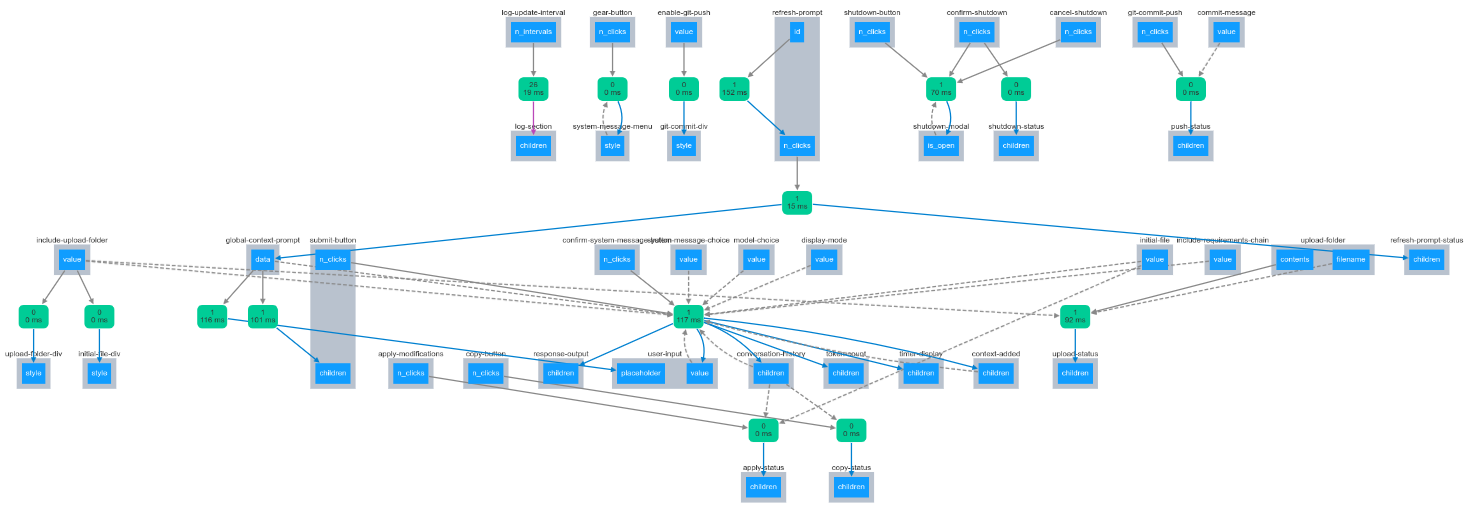
\includegraphics[height=0.6\textwidth, width=1.0\textwidth]{backend-callgraph.png}
  \caption{AGREE-Dog backend function call graph illustrating automated DevOps/ProofOps orchestration. Nodes represent key operations, while edges indicate dependencies and data flows between components.}
  \label{fig:callgraph}
\end{figure}

%%%%%
\pagebreak

%Memory Managment Subsystem
\begin{algorithm}[htbp]
\caption{Memory Management and Prompt Optimization in AGREE-Dog}
\label{alg:memory-management}
\SetKwInOut{Input}{Input}\SetKwInOut{Output}{Output}

\Input{User input, conversation state, AADL model repository, optional requirements file}
\Output{Optimized prompt, updated conversation history}

Initialize Short-Term, Temporary, and Long-Term memories\;

Identify and load recently updated files:
\begin{itemize}
    \item Identify recently updated files in repository.
    \item Load \textbf{only} these updated files into Temporary memory.
    \item Cache filenames and timestamps.
\end{itemize}

Integrate system-level requirements (if provided)\;

Construct prompt from:
\begin{itemize}
    \item Updated files from Temporary memory.
    \item User input and interaction history.
    \item System-level requirements.
\end{itemize}

Ensure prompt size within token limits (truncate oldest entries if necessary)\;

\textbf{Generate} response from AGREE-Dog model\;

Update Short-Term memory with latest interaction\;

\If{\textbf{User selects} \textit{Save Conversation}}{
    Save conversation to Long-Term memory\;
}

\If{\textbf{User selects} \textit{Commit to Git}}{
    Stage conversation and updated files\;
    Commit and push to remote repository\;
}

\textbf{return} optimized prompt, updated conversation history\;

\end{algorithm}

